\documentclass{../../../oss-ap12ibhl}

\begin{document}
\genheader

\gentitle{3}{WORK AND ENERGY}

\begin{questions}

  \question A \SI{1}{\kilo\gram} ball is thrown vertically downward from a
  50-meter-high tower with an initial speed of \SI{4}{\metre\per\second}. Just
  before striking the ground, the speed of the ball is
  \SI{20}{\metre\per\second}. The energy lost to air friction is most nearly
  \begin{choices}
    \choice\SI{101}{\joule}
    \choice\SI{210}{\joule}
    \choice\SI{308}{\joule}
    \choice\SI{406}{\joule}
    \choice\SI{508}{\joule}
  \end{choices}

  \question An archer pulls a bowstring back a distance of
  \SI{20}{\centi\metre} with an average force of \SI{75}{\newton}. The arrow
  has a mass of \SI{20.}{\gram}. When he releases the string, what is the
  velocity of the arrow when it leaves the bow?
  \begin{choices}
    \choice\SI{1.2}{\metre\per\second}
    \choice\SI{22}{\metre\per\second}
    \choice\SI{32}{\metre\per\second}
    \choice\SI{39}{\metre\per\second}
    \choice\SI{42}{\metre\per\second}
  \end{choices}
  
  % THESE TWO QUESTIONS ARE ALSO IN THE AP C HOMEWORK. MAY BE WE CAN CHANGE
  % SOMETHING LATER
  \uplevel{
    \textbf{Questions \ref{q:pq1}--\ref{q:pq2}}

    A \SI{2}{\kilo\gram} projectile is launched with a speed of
    \SI{20}{\metre\per\second} from horizontal ground at an angle of \ang{37}
    to the horizontal as shown. Point $P$ is at the top of the path, and point
    $Q$ is at the end of the path, just before the projectile again reaches the
    ground.
    \cpic{.35}{symprojectile}
  }

  \question The kinetic energy of the projectile at point $P$ is
  \label{q:pq1}
  \begin{choices}
    \choice\SI{108}{\joule}
    \choice\SI{225}{\joule}
    \choice\SI{256}{\joule}
    \choice\SI{400}{\joule}
    \choice\SI{525}{\joule}
  \end{choices}
    
  \question The kinetic energy of the projectile at point $Q$ is
  \label{q:pq2}
  \begin{choices}
    \choice\SI{108}{\joule}
    \choice\SI{225}{\joule}
    \choice\SI{256}{\joule}
    \choice\SI{400}{\joule}
    \choice\SI{525}{\joule}
    \end{choices}
    
  \question If a projectile thrown directly upward reaches a maximum height $h$
  and spends a total time in the air of $T$ before returning to its original
  position, the average power of the gravitational force during the trajectory
  is
  \begin{choices}
    \choice $P=2mgh/T$
    \choice $P=-2mgh/T$
    \choice 0
    \choice $P=mgh/T$
    \choice $P=-mgh/T$
  \end{choices}
    
  \question Given that the constant net force on an object and the object's 
  displacement, which of the following quantities can be calculated?
  \begin{choices}
    \choice the net change in the object's velocity
    \choice the net change in the object's mechanical energy
    \choice the average acceleration
    \choice the net change in the object's kinetic energy
    \choice the net change in the object's potential energy
  \end{choices}
    
  \question An electron travels in a circle around a hydrogen nucleus at a very
  high speed. The work done by the electrostatic force acting on the electron
  after one complete revolution is
  \begin{choices}
    \choice zero
    \choice positive
    \choice negative
    \choice equal to the kinetic energy of the electron
    \choice equal to the potential energy of the electron
  \end{choices}
    
  \question An object is moved from rest at point $P$ to rest at point $Q$ in a
  gravitational field. The net work against the gravitational field depends
  on the
  \begin{choices}
    \choice mass of the object and the positions of $P$ and $Q$
    \choice mass of the object only
    \choice positions of $P$ and $Q$ only
    \choice length moved between points $P$ and $Q$
    \choice coefficient of friction
  \end{choices}
    
  \question A pendulum bob of mass $m$ is released from rest as shown in the
  figure below. What is the tension in the string as the pendulum swings
  through the lowest point of its motion?

  \begin{minipage}{.4\linewidth}
    \begin{center}
      \begin{tikzpicture}[scale=.95]
        \draw[dashed](0,0)--(0,-3.5);
        \begin{scope}[rotate=60]
          \draw(0,0)--(0,-4);
          \fill[black](0,-4) circle(.13) node[right]{\tiny $m$};
          \draw[<->](.5,0)--(.5,-4) node[midway,above right]{\tiny $l$};
        \end{scope}
        \draw[<->](0,-1)arc(270:330:1) node[pos=.6,below]{\tiny\ang{60}};
      \end{tikzpicture}
    \end{center}
  \end{minipage}
  \begin{minipage}{.4\linewidth}
    \begin{choices}
      \choice $T=\dfrac12mg$
      \choice $T=mg$
      \choice $T=\dfrac32mg$
      \choice $T=2mg$
      \choice None of the above
    \end{choices}
  \end{minipage}
  \vspace{.7in}
    
%  \question Two blocks of mass $m_A$ and $m_B$ are connected by a string that
%  passes over a light pulley. The mass of $A$ is larger than the mass of $B$.
%  The speed of mass $A$ just before reaching the floor is:
%
%  \begin{minipage}{.4\linewidth}
%      \pic{.9}{pulley-a-b}
%  \end{minipage}
%  \begin{minipage}{.4\linewidth}
%    \begin{choices}
%      \choice $\sqrt{\dfrac{m_A-m_B}{m_A+m_B}gD}$
%      \choice $\sqrt{\dfrac{m_A+m_B}{m_A-m_B}gD}$
%      \choice $\sqrt{\dfrac{m_A}{m_A+m_B}gD}$
%      \choice $\sqrt{\dfrac{m_B}{m_A+m_B}gD}$
%      \choice $\sqrt{\dfrac{m_A}{m_B}gD}$
%    \end{choices}
%  \end{minipage}

  \uplevel{
    \textbf{Questions \ref{q:down1}--\ref{q:down2}}

    A force is applied to a block of mass $m$ at a downward angle of $\theta$
    to the vertical as shown. The block moves with a constant speed across a
    rough floor for a distance $x$.
    \begin{center}
      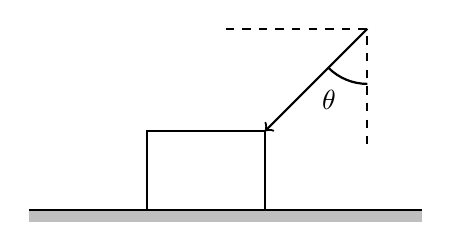
\begin{tikzpicture}
        \fill[gray!50](0,-.15) rectangle(5,0);
        \draw[thick](0,0)--(5,0);
        \draw[thick](1.5,0)rectangle(3,1);
        \draw[<-,thick](3,1)--(4.3,2.3);
          \draw[thick,dashed](2.5,2.3)--(4.3,2.3)--(4.3,.8);
          \draw[thick](4.3,1.6) arc(270:225:.7)
          node[midway,below left]{$\theta$};
      \end{tikzpicture}
    \end{center}
  }

  \question The work done by the applied force on the block is
  \label{q:down1}
  \begin{choices}
    \choice $Fx\sin\theta$
    \choice $Fx\cos\theta$
    \choice $Fmx\sin\theta$
    \choice $Fmx\cos\theta$
    \choice zero
  \end{choices}
    
  \question The coefficient of friction between the block and the floor is
  \label{q:down2}
  \begin{choices}
    \choice $\dfrac{F}{mg}$
    \choice $\dfrac{F\cos\theta}{mg}$
    \choice $\dfrac{F\cos\theta}{F\sin\theta+mg}$
    \choice $\dfrac{F\sin\theta}{F\cos\theta+mg}$
    \choice $\dfrac{F\cos\theta}{F\sin\theta}$
  \end{choices}

  \uplevel{
    \textbf{Questions \ref{sphere1}--\ref{sphere2}}

    A small block rests on the top of a smooth sphere of radius $R$ when it is
    given a light tap so that it just begins sliding on the sphere. When the
    block reaches the angle $\theta$, it loses contact with the surface of the
    sphere.
    \begin{center}
      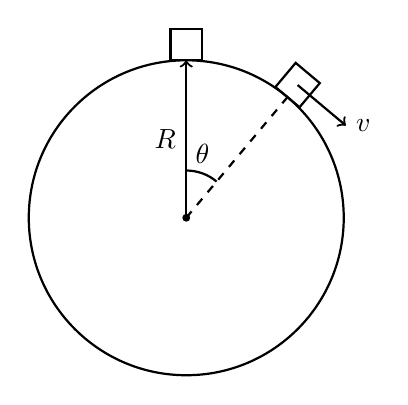
\begin{tikzpicture}
        \draw[thick](0,0) circle(2);
        \fill(0,0) circle(.05);
        \draw[thick,->](0,0)--(0,2) node[midway,left]{$R$};
        \draw[thick](-.2,2) rectangle(.2,2.4);
        \begin{scope}[rotate around={-40:(0,0)}]
          \draw[thick,dashed](0,0)--(0,2);
          \draw[thick](-.2,2) rectangle(.2,2.4);
          \draw[->,thick](0,2.2)--(.8,2.2) node[right]{$\bm{v}$};
        \end{scope}
        \draw[thick](0,.6) arc(90:50:.6) node[midway,above]{$\theta$};
      \end{tikzpicture}
    \end{center}
  }

  \question The kinetic energy of the block as it leaves the surface of the
  sphere is
  \label{sphere1}
  \begin{choices}
    \choice $mgR$
    \choice $mgR\cos\theta$
    \choice $mgR\sin\theta$
    \choice $mg(R-R\cos\theta)$
    \choice $mg(R-R\sin\theta)$
  \end{choices}

  \question The speed of the block as it leaves the surface of the sphere is
  \label{sphere2}
  \begin{choices}
    \choice $\displaystyle\sqrt{2g}{m}$
    \choice $\displaystyle\sqrt{2gR}{m}$
    \choice $\displaystyle 2gR\cos\theta$
    \choice $\displaystyle 2g(R-R\cos\theta)$
    \choice $\displaystyle 2g(R-R\sin\theta)$
  \end{choices}
    
  \question A small ball starts from rest and rolls down a quarter-circle ramp
  of radius $R$. The speed of the ball at the point halfway down the ramp is
  most nearly

  \begin{minipage}{.3\linewidth}
    \centering
    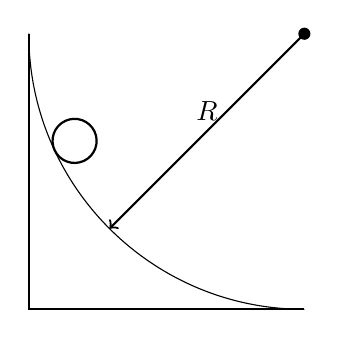
\begin{tikzpicture}[scale=3.5]
      \draw[thick](-1,0)--(-1,-1)--(0,-1);
      \draw(-1,0) arc(180:270:1);
      \draw[thick,->,rotate=45](0,0)--(-1,0) node[midway,above,sloped]{$R$};
      \draw[thick,rotate=25](-.92,0) circle(.08);
      \fill (0,0) circle(.022);
    \end{tikzpicture}
  \end{minipage}
  \begin{minipage}{.68\linewidth}
    \begin{choices}
      \choice $gR$
      \choice $2gR$
      \choice $\displaystyle\sqrt{gR\sin\ang{45}}$
      \choice $\displaystyle\sqrt{2gR\sin\ang{45}}$
      \choice The speed cannot be determined without knowing the mass of the
      ball.
    \end{choices}
  \end{minipage}
  \newpage
  
  \uplevel{
    \cpic{.45}{pendulum}
  }

  \question A simple pendulum consists of a bob of mass 1.8 kg attached to a
  string of length \SI{2.3}{\metre}. The pendulum is held at an angle of
  \ang{30} from the vertical by a light horizontal string attached to a wall,
  as shown above.
  \begin{parts}
    \part On the figure below, draw a free-body diagram showing and labeling the
    forces on the bob in the position shown above.
    \begin{center}
      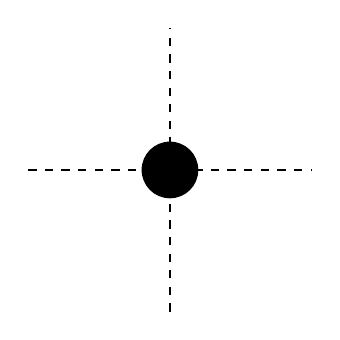
\begin{tikzpicture}[scale=.9]
        \draw[dashed](-2,0)--(2,0);
        \draw[dashed](0,-2)--(0,2);
        \fill(0,0) circle(.4);
      \end{tikzpicture}
    \end{center}
    \part Calculate the tension in the horizontal string.
    \part The horizontal string is now cut close to the bob, and the pendulum
    swings down. Calculate the speed of the bob at its lowest position.
  \end{parts}
  \newpage

  \uplevel{
    \centering
    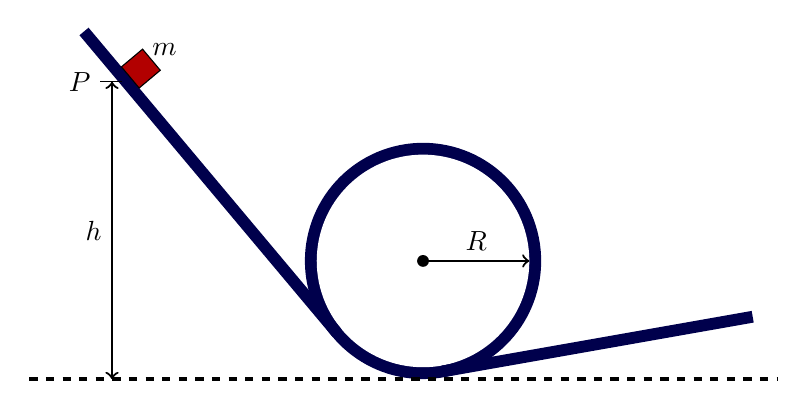
\begin{tikzpicture}[scale=.5]
      \fill[blue!30!black](0,0) circle(3);
      \fill[white](0,0) circle(2.7);
      \fill[black](0,0) circle(.15);
      \draw[thick,->](0,0)--(2.7,0) node[midway,above]{$R$};
      \begin{scope}[rotate=10]
        \fill[blue!30!black](0,-2.7) rectangle(8,-3);
      \end{scope}
      \begin{scope}[rotate=-50]
        \fill[blue!30!black](0,-2.7) rectangle(-10,-3);
        \fill[red!70!black,draw=black](-8,-2.7) rectangle(-8.7,-2)
        node[right,black]{$m$};
      \end{scope}
      \draw[dashed,very thick](-10,-3)--(9,-3);
      \draw[thick,<->](-7.9,-3)--(-7.9,4.55) node[midway,left]{$h$};
      \draw(-7.65,4.55)--(-8.2,4.55) node[left]{$P$};    
    \end{tikzpicture}
  }

  \question A small block of mass $m$ slides without friction along the
  loop-the-loop track shown in the figure above. The block starts from point
  $P$ a distance $h$ above the bottom of the loop.
  \begin{parts}
    \part What is the kinetic energy of the block when it reaches the top of
    the loop?
    \part What is the acceleration at the top of the loop, assuming that it
    stays on the track?
    \part What is the least value of $h$ for which the block will reach the top
    of the loop without leaving the track?
  \end{parts}
  \newpage

  \uplevel{
    \centering
    \begin{tikzpicture}[scale=.7]
      \begin{scope}[rotate=-30]
        \fill(0,0) rectangle(-.1,1);
        \draw[thick,
          decoration={aspect=.4,segment length=1.5mm, amplitude=2mm,coil},
          decorate] (-.1,.5)--(-1.5,.5)
        node[midway,above right]{$k=\SI{100}{\newton\per\metre}$};
        \fill(-1.5,0) rectangle(-1.6,1);
        \draw[<->,thick](-1.6,1.5)--(-5.6,1.5)
        node[midway,above right,sloped]{\SI{4.}{\metre}};
        \draw[thick](-1.6,1.05)--(-1.6,2);
        \draw[thick](-5.6,1.05)--(-5.6,2);
        \draw[fill=yellow!50](-5.6,0) rectangle(-6.3,.7)
        node[black,above left]{$m=\SI{2.}{\kilo\gram}$};
      \end{scope}
      \draw[fill=pink!50](0,0)--(-6.06,0)--(-6.06,3.5)--cycle;
      \draw[<->,thick](-2,0) arc(180:150:2) node[midway,left]{\ang{30}};
    \end{tikzpicture}
  }
  \question A \SI{2}{\kilo\gram} block is released \SI{4.}{\metre} from a
  massless spring with a spring constant of \SI{100}{\newton\per\metre} that is
  fixed along a frictionless plane inclined at \ang{30}, as shown in the figure
  below. Plese give answer to $3$ significant figures.
  \begin{parts}
    \part Find the maximum compression of the spring.
    \part If the plane is not frictionless, and the coefficient of kinetic
    friction between it and the block is $0.20$, find the maximum compression.
    \part For the rough incline ($\mu=0.20$), how far up the incline will the
    block travel after leaving the spring?
  \end{parts}
  \newpage

  \uplevel{
    \cpic{.8}{table}
  }
  
  \question A physics class is asked to design a low-friction slide that will
  launch a block horizontally from the top of a lab table. Teams 1 and 2
  assemble the slides shown above and use identical blocks 1 and 2,
  respectively. Both slides start at the same height $d$ above the tabletop.
  However, team 2's table is lower than team 1's table. To compensate for the
  lower table, team 2 constructs the right end of the slide to rise above the
  tabletop so that the block leaves the slide horizontally at the same height
  $h$ above the floor as does team 1's block (see figure above).
  \begin{parts}
    \part Both blocks are released from rest at the top of their respective
    slides. Do block 1 and block 2 land the same distance from their respective
    tables? Justify your answer.

    \vspace{.1in}
    \underline{\hspace{.3in}} Yes\hspace{.2in}
    \underline{\hspace{.3in}} No

    \vspace{.1in}
    \uplevel{
      In another experiment, teams 1 and 2 use tables and low-friction slides
      with the same height. However, the two slides have different shapes, as
      shown below.
      \cpic{.8}{table2}
    }

    \part Both blocks are released from rest at the top of their respective
    slides at the same time.
    \begin{subparts}
      \subpart Which block, if either, lands farther from its respective table?
      Briefly explain your reasoning without manipulating equations.
      
      \vspace{.1in}
      \underline{\hspace{.3in}} Block 1
      \underline{\hspace{.3in}} Block 2
      \underline{\hspace{.3in}} The two blocks land the same distance from
      their respective tables.

      \vspace{.1in}
      
      \subpart Which block, if either, hits the floor first? Briefly explain
      your reasoning without manipulating equations.
      \vspace{.1in}
      \underline{\hspace{.3in}} Block 1\hspace{.3in}
      \underline{\hspace{.3in}} Block 2\hspace{.3in}
      \underline{\hspace{.3in}} The two blocks hit the floor at the same time.
    \end{subparts}
  \end{parts}
  \newpage

  \uplevel{
    \cpic{.4}{pendulum-peg}
  }
  
  \question A pendulum of length $L$ has a bob of mass $m$. It is released from
  some angle $\theta_1$. The string hits a peg at a distance $x$ directly below
  the pivot, as shown in the figure below, effectively shortening the length of
  the pendulum. Find the maximum angle $\theta_2$ between the string and the
  vertical when the bob is to the right of the peg.
\end{questions}
\end{document}
